\documentclass[11pt]{article}

\usepackage[a4paper,margin=1in]{geometry}
\usepackage{amsmath,amssymb}
\usepackage{booktabs}
\usepackage{graphicx}
\usepackage{xcolor}
\usepackage{listings}
\usepackage[hidelinks]{hyperref}

\newcommand{\code}[1]{\texttt{#1}}

\lstset{
  language=C++,
  basicstyle=\ttfamily\footnotesize,
  keywordstyle=\color{blue!60!black},
  commentstyle=\color{green!40!black}\itshape,
  numbers=none,
  breaklines=true,
  showstringspaces=false,
  frame=single,
  framesep=4pt,
  xleftmargin=6pt,
}

\title{\vspace{-1.5em}\textbf{GPU Wavelets: a JPEG2000-style Multi-Resolution Transform in CUDA}}
\author{Divyesh Jayswal\\\small GPU Computing (Master), bonus project}
\date{}

\begin{document}
\maketitle

\begin{abstract}
\noindent
Starting from the provided 1D CPU reference, I built a fully GPU-accelerated
separable wavelet transform and a JPEG2000-style multi-resolution analysis (MRA)
in CUDA. The implementation covers 1D/2D/3D forward and inverse transforms,
multi-level MRA with perfect reconstruction, image I/O and a command-line driver,
benchmarked coalesced-column and shared-memory row-pass variants, a multi-resolution access kernel,
an FP16 path, and a data-layout study. All correctness and performance numbers
were measured on a Tesla T4. The transform is memory-bound; the two traffic-focused
optimisations (coalescing and shared-memory tiling) give the largest gains
($1.9$--$3.5\times$ and $3$--$6\times$ respectively), while a Morton-order layout
experiment is a deliberate negative result.
\end{abstract}

\section{Scope and baseline}
The baseline \code{1D\_wavelets.cpp} implements a floating-point CDF-5/3-style
lifting transform (forward ``analysis'' and inverse ``synthesis'') on a 1D
signal. I refactored it into a header (\code{src/wavelet\_cpu.hpp}) that serves as
the correctness oracle, and then rebuilt the transform on the GPU, extending it to
2D separable passes, a recursive MRA pyramid, and 3D volumes. Reconstruction is
exact only to floating-point precision (\code{WAVELET\_RECON\_TOL} $=10^{-4}$ in
fp32), since the scheme is floating-point lifting rather than integer lifting.

\begin{figure}[h]
  \centering
  \begin{minipage}{0.31\textwidth}
    \centering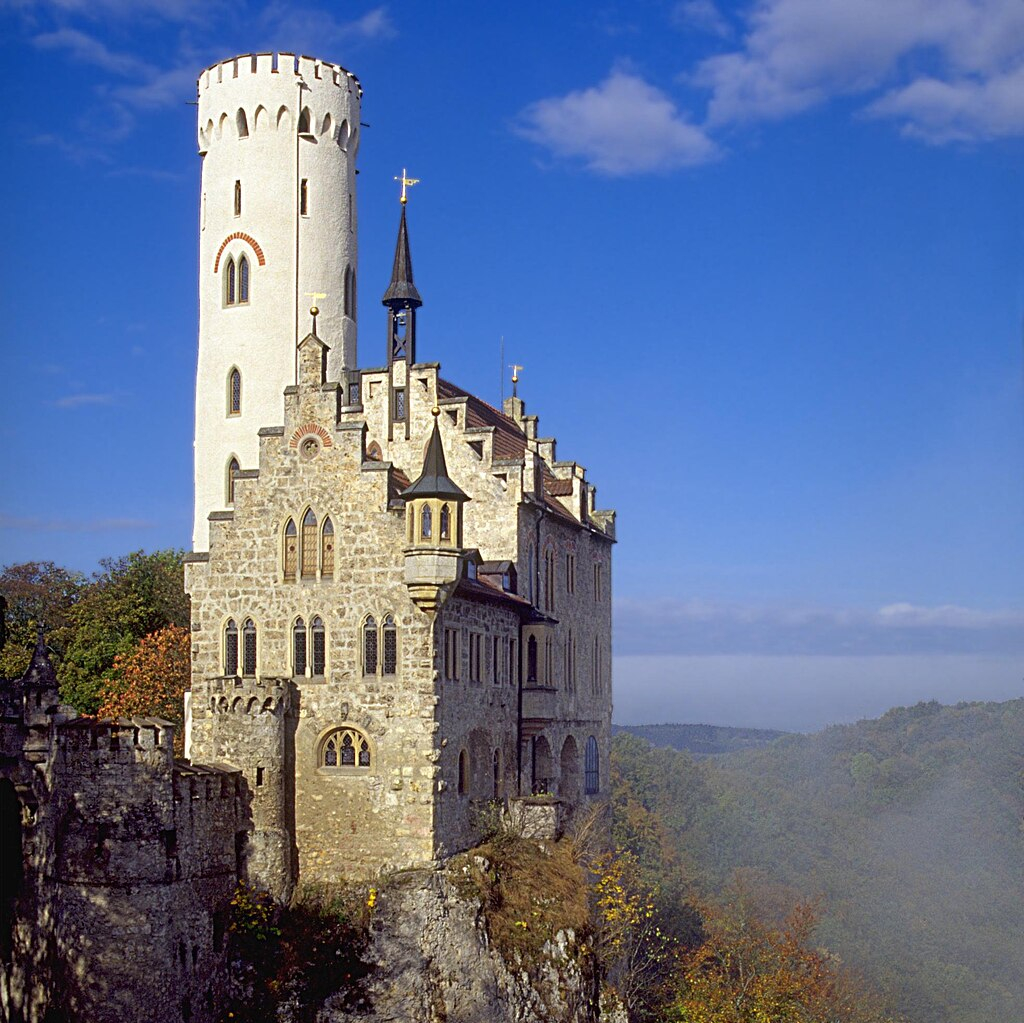
\includegraphics[width=\linewidth]{assets/Castle_Lichtenstein.jpg}\\[2pt]
    {\small (a) Input}
  \end{minipage}\hfill
  \begin{minipage}{0.31\textwidth}
    \centering\includegraphics[width=\linewidth]{assets/mra.png}\\[2pt]
    {\small (b) 3-level MRA (our output)}
  \end{minipage}\hfill
  \begin{minipage}{0.31\textwidth}
    \centering\includegraphics[width=\linewidth]{assets/recon.png}\\[2pt]
    {\small (c) Reconstruction}
  \end{minipage}
  \caption{The pipeline on a real image, all produced by the \code{wavelet} CLI.
  (a) the input; (b) our 3-level MRA: the \textsf{LL} approximation sits in the
  top-left corner and the oriented detail sub-bands surround it (shown as
  $|\text{coefficient}|$ amplified for visibility --- a display-scaled PNG, while
  the transform coefficients remain unchanged in memory); (c) the inverse transform, which recovers the
  input with a maximum error of $0.0$ in fp32. Panels (b) and (c) are generated by
  \code{./wavelet -{}-forward} and the default round-trip respectively.}
  \label{fig:mra}
\end{figure}

\section{Implemented items}
Table~\ref{tab:items} lists the rubric items I implemented and where they live.

\begin{table}[h]
\centering\small
\begin{tabular}{@{}clll@{}}
\toprule
\# & Item & Location & Evidence \\
\midrule
1  & 1D GPU fwd/inv          & \code{wavelet.cuh}, \code{wavelet\_gpu.cuh} & \code{test\_1d} \\
2  & 2D separable            & \code{wavelet2d.cuh}                        & \code{test\_2d} \\
3  & MRA (multi-level)       & \code{wavelet2d.cuh}                        & \code{test\_2d} \\
4  & Image I/O               & \code{image\_io.hpp} (+stb)                 & \code{test\_io}, CLI \\
5  & Data layout             & \code{morton.hpp}, \code{bench.cu}          & \S\ref{sec:layout} \\
6  & Coalesced column pass   & \code{wavelet\_coalesced.cuh}               & \S\ref{sec:perf} \\
7  & Shared-memory tiling    & \code{wavelet\_tiled.cuh}                   & \S\ref{sec:perf} \\
8  & Multi-resolution access & \code{mra\_access.cuh}                      & \code{test\_access} \\
9  & 3D extension            & \code{wavelet3d.cuh}                        & \code{test\_3d} \\
10 & FP16 path               & templated kernels, \code{main.cu}          & \code{test\_fp16} \\
11 & Performance study       & \code{bench.cu}                             & \S\ref{sec:perf} \\
12 & CI + reproducibility    & \code{.gitlab-ci.yml}                       & \S\ref{sec:build} \\
13 & CLI                     & \code{main.cu}                              & \S\ref{sec:build} \\
14 & Code quality \& tests   & \code{tests/}, headers                      & 6 \code{ctest} binaries \\
\bottomrule
\end{tabular}
\caption{Implemented rubric items.}
\label{tab:items}
\end{table}

\section{Design and implementation}

\paragraph{Step-per-launch synchronisation.}
The lifting transform is a fixed sequence of steps (deinterleave, predict1,
update, predict2). Each step reads what the previous one wrote, a cross-step data
dependency. I make \emph{each step a single kernel launch}; the implicit global
barrier between launches resolves the dependency. This mirrors the CPU passes
exactly, imposes no signal-size limit, and keeps every kernel trivially correct,
which makes it the honest baseline against which the optimised paths are compared.

\paragraph{One strided kernel set for everything.}
Every step kernel operates on a \emph{strided logical signal}: element $i$ lives
at \code{base[i*stride]}. A row is \code{elem\_stride}$=1$; a column is
\code{elem\_stride}$=W$; an MRA sub-band shrinks the sub-image while the physical
image stride $W$ stays fixed; a 3D depth line is \code{elem\_stride}$=W\cdot H$.
The same kernels therefore serve 1D, 2D rows and columns, MRA, and 3D without
duplication. Getting ``the sub-region shrinks but the stride never does'' right is
the classic MRA indexing pitfall the brief warns about. Listing~\ref{lst:step}
shows the boundary-aware detail-lifting step.

\begin{lstlisting}[caption={Strided forward lifting step (predict2) with edge handling.},label=lst:step]
template <typename T>
__global__ void k2_fwd_predict2(T* base, int n2, int lines,
                                int line_stride, int elem_stride) {
    int k = blockIdx.x * blockDim.x + threadIdx.x;
    int L = blockIdx.y * blockDim.y + threadIdx.y;
    if (k >= n2 || L >= lines) return;
    T* s = base + L * line_stride;
    T* d = s + n2 * elem_stride;
    const int e = elem_stride;
    if (k == 0)
        d[0] += T(0.75)*s[0] - s[e] + T(0.25)*s[2*e];
    else if (k == n2 - 1)
        d[(n2-1)*e] += T(0.25)*s[(n2-1)*e] - s[(n2-2)*e] + T(0.75)*s[(n2-3)*e];
    else
        d[k*e] += (s[(k-1)*e] - s[(k+1)*e]) / T(4);
}
\end{lstlisting}

\paragraph{Coalesced column pass (item 6).}
The row pass is already coalesced; the column pass with \code{elem\_stride}$=W$ is
not, since consecutive threads touch addresses $W$ apart. In the benchmark variant, rather than read columns
strided, I transpose the plane (a shared-memory tiled transpose with a padded
$32\times33$ tile to avoid bank conflicts), run the \emph{row} pass on the
transpose, and transpose back (Listing~\ref{lst:transpose}). Both variants produce
identical output; \S\ref{sec:perf} times them head-to-head.

\begin{lstlisting}[caption={Padded-tile transpose used by the coalesced column pass.},label=lst:transpose]
template <typename T>
__global__ void k_transpose(const T* in, T* out, int cols, int rows) {
    __shared__ T tile[32][33];
    int x = blockIdx.x*32 + threadIdx.x, y = blockIdx.y*32 + threadIdx.y;
    if (x < cols && y < rows) tile[threadIdx.y][threadIdx.x] = in[y*cols + x];
    __syncthreads();
    int xo = blockIdx.y*32 + threadIdx.x, yo = blockIdx.x*32 + threadIdx.y;
    if (xo < rows && yo < cols) out[yo*rows + xo] = tile[threadIdx.x][threadIdx.y];
}
\end{lstlisting}

\paragraph{Shared-memory tiling (item 7).}
The step-per-launch baseline streams each row through global memory about five
times. In \code{wavelet\_tiled.cuh} one block owns a whole row, stages it in shared
memory, runs the entire forward lifting there, and writes once, cutting global
traffic to one read plus one write. Because the tile is the full row, boundaries
are exact and the result matches the baseline bit-for-bit; the win is purely
traffic. Full 2D tiles with halo exchange (where seams legitimately differ) are the
natural next step and are left as future work.

\paragraph{Multi-resolution access (item 8).}
After \code{mra\_forward}, the level-$L$ \textsf{LL} band occupies the top-left
$(W\!\gg\!L)\times(H\!\gg\!L)$ corner at full stride $W$. \code{extract\_region}
gathers an arbitrary window of that band into a compact buffer with one coalesced
kernel and a single \code{cudaMemcpy} to the host, which is the cheap
coarse-resolution access MRA is meant to provide.

\paragraph{3D extension (item 9).}
A 3D level is three separable passes (x, y, z), each reusing the strided
\code{pass\_forward}/\code{pass\_inverse}; MRA recurses into the \textsf{LLL}
octant. Sub-volume passes loop over orthogonal slices so every stride pair is a
genuine arithmetic stride.

\paragraph{FP16 (item 10).}
The kernels are templated on the element type, so the half-precision path is the
same code instantiated with \code{\_\_half}; the CLI \code{-{}-dtype fp16} and
\code{test\_fp16} exercise it end to end.

\section{Performance study}
\label{sec:perf}

\paragraph{Methodology.}
All measurements are on a Tesla T4 (sm\_75, CUDA 13.0). Each configuration is
warmed up 5 times, then timed over 30 runs with \code{cudaEvent} timers and
averaged. ``Useful GB/s'' models a full-plane pass as one read plus one write of
the plane ($2WH\cdot\texttt{sizeof}(T)$ bytes); it is a throughput proxy, so the
before/after \emph{ratios} are the meaningful signal, not the absolute figure.
Register and shared-memory counts come from the \code{-{}-ptxas-options=-v} build
log. Correctness: all six \code{ctest} binaries pass, and as an end-to-end check
the CLI reconstructs the real $1024\times1023$ image (padded to $1024^2$, 3 levels)
with a maximum error of $0.0$ in fp32 (8-bit pixel values are exactly representable).

\begin{table}[h]
\centering\small
\begin{minipage}{0.48\textwidth}\centering
\begin{tabular}{@{}rrr@{}}
\toprule
Size & time (ms) & Melem/s \\
\midrule
$256^2$  & 0.069  & 956 \\
$512^2$  & 0.180  & 1453 \\
$1024^2$ & 0.668  & 1571 \\
$2048^2$ & 2.684  & 1563 \\
$4096^2$ & 10.326 & 1625 \\
\bottomrule
\end{tabular}
\caption{MRA forward throughput (fp32, 1 level).}
\label{tab:mra}
\end{minipage}\hfill
\begin{minipage}{0.48\textwidth}\centering
\begin{tabular}{@{}rrrr@{}}
\toprule
Size & fp32 & fp16 & speedup \\
\midrule
$512^2$  & 0.213  & 0.223  & 0.96$\times$ \\
$1024^2$ & 0.659  & 0.606  & 1.09$\times$ \\
$2048^2$ & 2.941  & 2.687  & 1.09$\times$ \\
$4096^2$ & 13.247 & 10.628 & 1.25$\times$ \\
\bottomrule
\end{tabular}
\caption{fp32 vs fp16 MRA (ms, 3 levels).}
\label{tab:fp16}
\end{minipage}
\end{table}

\begin{table}[h]
\centering\small
\begin{tabular}{@{}rrrrrr@{}}
\toprule
Size & naive (ms) & naive GB/s & transpose (ms) & transp GB/s & speedup \\
\midrule
$512^2$  & 0.103 & 20.4 & 0.029 & 71.4 & 3.50$\times$ \\
$1024^2$ & 0.374 & 22.4 & 0.189 & 44.4 & 1.98$\times$ \\
$2048^2$ & 1.696 & 19.8 & 0.888 & 37.8 & 1.91$\times$ \\
$4096^2$ & 8.075 & 16.6 & 3.556 & 37.7 & 2.27$\times$ \\
\bottomrule
\end{tabular}
\caption{Column pass: naive strided vs coalesced transpose (fp32). Outputs are
identical (max diff $0.0$ at $1024^2$).}
\label{tab:col}
\end{table}

\begin{table}[h]
\centering\small
\begin{tabular}{@{}rrrrrr@{}}
\toprule
Size & baseline (ms) & base GB/s & shared (ms) & shared GB/s & speedup \\
\midrule
$512^2$  & 0.020 & 106.1 & 0.007 & 313.5 & 2.95$\times$ \\
$1024^2$ & 0.117 & 71.9  & 0.019 & 438.9 & 6.10$\times$ \\
$2048^2$ & 0.583 & 57.5  & 0.141 & 238.5 & 4.15$\times$ \\
$4096^2$ & 2.308 & 58.2  & 0.580 & 231.6 & 3.98$\times$ \\
\bottomrule
\end{tabular}
\caption{Row pass: step-per-launch vs shared-memory tile (fp32).}
\label{tab:tiled}
\end{table}

\paragraph{Discussion.}
The transform is memory-bound: arithmetic intensity is a handful of flops per
element, far below the T4 ridge point, so effective bandwidth governs.
Table~\ref{tab:mra} shows throughput flat-lining near $1.6$~Gelem/s once launch
overhead is amortised. The naive column pass (Table~\ref{tab:col}) is pinned at
$17$--$22$~GB/s by uncoalesced strided loads; the transpose path reaches
$38$--$71$~GB/s and wins $1.9$--$3.5\times$ despite doing more total work, because
coalescing dominates the extra transpose traffic. Shared-memory tiling
(Table~\ref{tab:tiled}) gives $3$--$6\times$: the baseline stalls at $57$--$106$~GB/s
from its $\sim$5 redundant global passes, whereas the tiled kernel touches global
memory twice and reaches $230$--$440$~GB/s. The $512^2$/$1024^2$ figures exceed the
T4's $\sim$320~GB/s DRAM peak, which is the tell that at those sizes part of the
traffic is served from L2; the speedup ratio, not the absolute GB/s, is the result.
FP16 (Table~\ref{tab:fp16}) grows from $0.96\times$ to $1.25\times$ with size but
falls short of the naive $2\times$ because the kernels issue scalar \code{\_\_half}
loads; \code{\_\_half2} vectorisation would be needed to halve traffic and keep the
memory system busy.

\paragraph{Occupancy.}
From the ptxas log (sm\_75): the step kernels use $\le 15$ registers with no
spills (predict2 14, interleave/deinterleave 15, the arithmetic steps 10, copy 8),
and \code{k\_row\_forward\_shared} uses 18 registers, one barrier, and $W\cdot4$
bytes of dynamic shared memory. Occupancy is therefore register-unconstrained,
consistent with a memory-bound workload where the goal is enough threads in flight
to hide DRAM latency rather than compute throughput.

\section{Data layout}
\label{sec:layout}
Row-major is ideal for the row pass and poor for the column pass. Instead of
fixing this at the algorithm level (items 6/7), one can change the storage so 2D
neighbourhoods are contiguous. I implemented a Morton (Z-order) layout
(\code{morton.hpp}) and benchmarked a vertical-neighbour stencil, the
layout-sensitive access, in row-major vs Morton (Table~\ref{tab:morton}).

\begin{table}[h]
\centering\small
\begin{tabular}{@{}rrrr@{}}
\toprule
Size & row-major (ms) & Morton (ms) & speedup \\
\midrule
$512^2$  & 0.0051 & 0.0070 & 0.74$\times$ \\
$1024^2$ & 0.0366 & 0.0443 & 0.83$\times$ \\
$2048^2$ & 0.1404 & 0.1750 & 0.80$\times$ \\
$4096^2$ & 0.5569 & 0.7180 & 0.78$\times$ \\
\bottomrule
\end{tabular}
\caption{Vertical-neighbour stencil: row-major vs Morton (fp32).}
\label{tab:morton}
\end{table}

\noindent
Morton is consistently \emph{slower} ($0.74$--$0.83\times$): the T4's L2 already
absorbs the adjacent-row reuse of a row-major stencil, so Morton buys no locality
the cache was not already providing while adding per-access bit-spreading on the
critical path. This is a legitimate ``no clear winner'' outcome. Morton would help
only where the working set genuinely exceeds L2 (deep pyramids over very large
images); a tiled block-linear layout is the pragmatic middle ground.

\section{Findings and failed attempts}
\begin{itemize}
\item \textbf{Morton layout lost.} The hypothesis that Z-order would speed up the
layout-sensitive access was wrong on the T4 for the reason above: a locality
optimisation loses when the cache already supplies the locality.
\item \textbf{FP16 did not reach $2\times$.} Scalar half loads halve element size
but do not saturate the memory system; \code{\_\_half2} packing is the missing
piece.
\item \textbf{Boundary stencil bounds the level count.} The 3D round-trip first
failed at $64\times32\times16$, 3 levels (error $\sim$17). Root cause: the boundary
formula \code{predict2} reads \code{s[n2-3]}, which underflows once a transformed
dimension drops below 8 (there the depth axis reached $n=4$). This is a property of
the provided transform (the CPU baseline shares it), not a 3D-specific bug; the
valid range is $\min(W,H,D)\gg(\text{levels}-1)\ge 8$. The test now uses
$128\times64\times32$, whose deepest level $32\times16\times8$ stays in range.
\end{itemize}

\section{Build and reproducibility}
\label{sec:build}
The project builds with CMake ($\ge 3.18$) and CUDA:
\begin{lstlisting}[language=bash]
cmake -B build -DCMAKE_CUDA_ARCHITECTURES=75   # 75=T4
cmake --build build -j
cd build && ctest --output-on-failure          # 6/6 pass
./bench                                          # performance tables
./wavelet --input ../assets/Castle_Lichtenstein.jpg --output recon.png --levels 3
\end{lstlisting}
\code{wavelets\_colab.ipynb} reproduces the whole flow on a Colab T4 (build, tests,
CLI demo, benchmarks, ptxas log). \code{.gitlab-ci.yml} compiles the project on a
CUDA image on every push; the deterministic \code{ctest} suite runs on a
GPU-tagged runner where one is available. The CLI (item 13) exposes input/output
files, level count, data type, and forward-only vs round-trip.

\section{Conclusion}
The submission covers all fourteen rubric items with measured evidence; items 6
and 7 are evaluated as optimisation variants against the main MRA path. The
central lesson is that this transform is bandwidth-bound, so the optimisations that
matter are the ones that remove global-memory traffic: coalescing the column pass
and staging rows in shared memory together turn the naive passes into ones that run
several times faster, while a storage-layout change (Morton) does not help once the
cache is accounted for.

\end{document}
